\documentclass[final]{lmuposter}
%
% defaults for height, width and distance of boxes are defined in
% lmuposter for a 3x3 box poster the following variables are defined:
% \MyBoxHeight, \MyBoxWidth, \MyBoxHSep, \MyBoxVSep, \MyIntBoxSep
%
% helpful for justifying the boxes, use the following in the header:
%
\setlength{\parindent}{0pt}
%
% Fonts of package Latin
%
% German language
\usepackage[ngerman]{babel}
% Fonts of package UTF8
\usepackage[utf8x]{inputenc}
%\usepackage[latin1]{inputenc}
%\usepackage[T1]{fontenc}
%
% pgf and tikz for graphics
%
\usepackage{pgf}
\usepackage{pgflibrarysnakes}
\usepackage{tikz}

%
% mathematical symbols of the ams package
%
\usepackage{amsmath}
\usepackage{amssymb}
\usepackage{bbm}
%\usepackage{marvosym}

%
% macros for vectors, matrix and so on
%
%\newsavebox{\fmbox}
\newenvironment{fmpage}[1]
	{\begin{lrbox}{\fmbox}\begin{minipage}{#1}}
	{\end{minipage}\end{lrbox}\fbox{\usebox{\fmbox}}}
%
% Puts a algorithm environment
\newenvironment{algorithm}[1][]{%
	\begin{table}[h]
	\centering
	\begin{minipage}[t]{12cm}
	\hspace{\stretch{2}} {\caption{\label{#1} #1}}
	\rule[1.5ex]{12cm}{0.01cm}\\
	%\hspace{\stretch{2}} {\tiny \textsc{ #1}}}
	\hspace{\stretch{2}} \\
	% SPACE BEFORE \\ IS IMPORTANT, ELSE NO STRETCHING
	\vspace{-4ex}
	\begin{list}{#1}{\labelwidth=12em \leftmargin=120pt}
	\vspace{-1ex}
}{%
	\end{list}
	\rule[1ex]{12cm}{0.01cm}\\
	\end{minipage}
	\vspace{-2ex}
	\end{table}
}
%
\newcommand{\atem}[2]{\item[\texttt{#1}] #2\vspace{1ex}}
%
% Some math stuff, you need to include \usepackage{amsmath} 
%
%
%\mathop is needed to  get the spacing correct,
%
\newcommand{\sign}{\mathop{\mathrm{sign}}}
%
% greek symbols are displayed fat, too 
%
\renewcommand{\vector}[1]{\boldsymbol{#1}}
%
% use straight letters for matrixes
%
\renewcommand{\matrix}[1]{\mathbf{#1}}
%
% Some further definitions
%
\newcommand{\set}[1]{\mathbb{#1}}
\newcommand{\transpose}{\mathsf{T}}
\newcommand{\unity}{\mathbbm{1}}


%needed for inline lists:
\usepackage{paralist}

\usepackage{verbatim}
% Python listing setup
\usepackage{color}
\usepackage[procnames]{listings}
\usepackage{setspace}
\renewcommand{\lstlistlistingname}{Code Listings}
\renewcommand{\lstlistingname}{Code Listing}
\definecolor{gray}{gray}{0.5}
\definecolor{lightgray}{gray}{0.9}
\definecolor{green}{rgb}{0,0.5,0}
\definecolor{lightgreen}{rgb}{0,0.7,0}
\definecolor{orange}{rgb}{1,0.5,0}
\definecolor{purple}{rgb}{0.5,0,0.5}
\definecolor{darkred}{rgb}{0.5,0,0}


\lstset{
language=python,
extendedchars=true,
%basicstyle=\ttfamily\small\setstretch{1},
basicstyle=\footnotesize,
mathescape=true,
breaklines=true,
numbers=left,
numbersep=10pt,
numberstyle=\tiny,
framexleftmargin=30pt,
xleftmargin=55pt,
stringstyle=\color{green},
showstringspaces=false,
alsoletter={1234567890},
otherkeywords={\ , \}, \{},
keywordstyle=\color{blue},
emph={access,and,as,break,class,continue,def,del,elif,else,%
except,exec,finally,for,from,global,if,import,in,is,%
lambda,not,or,pass,print,raise,return,try,while,assert},
emphstyle=\color{orange}\bfseries,
emph={[2]self},
emphstyle=[2]\color{gray},
emph={[4]ArithmeticError,AssertionError,AttributeError,BaseException,%
DeprecationWarning,EOFError,Ellipsis,EnvironmentError,Exception,%
False,FloatingPointError,FutureWarning,GeneratorExit,IOError,%
ImportError,ImportWarning,IndentationError,IndexError,KeyError,%
KeyboardInterrupt,LookupError,MemoryError,NameError,None,%
NotImplemented,NotImplementedError,OSError,OverflowError,%
PendingDeprecationWarning,ReferenceError,RuntimeError,RuntimeWarning,%
StandardError,StopIteration,SyntaxError,SyntaxWarning,SystemError,%
SystemExit,TabError,True,TypeError,UnboundLocalError,UnicodeDecodeError,%
UnicodeEncodeError,UnicodeError,UnicodeTranslateError,UnicodeWarning,%
UserWarning,ValueError,Warning,ZeroDivisionError,abs,all,any,apply,%
basestring,bool,buffer,callable,chr,classmethod,cmp,coerce,compile,%
complex,copyright,credits,delattr,dict,dir,divmod,enumerate,eval,%
execfile,exit,file,filter,float,frozenset,getattr,globals,hasattr,%
hash,help,hex,id,input,int,intern,isinstance,issubclass,iter,len,%
license,list,locals,long,map,max,min,object,oct,open,ord,pow,property,%
quit,range,raw_input,reduce,reload,repr,reversed,round,set,setattr,%
slice,sorted,staticmethod,str,sum,super,tuple,type,unichr,unicode,%
vars,xrange,zip},
emphstyle=[4]\color{purple}\bfseries,
morecomment=[s][\color{lightgreen}]{"""}{"""},
morekeywords={and,as,assert,break,class,continue,def,del,elif,else,except,
     finally,for,from,global,if,import,in,is,lambda,not,or,pass,print,
     return,try,while,with,yield},
commentstyle=\color{red}\slshape,
%literate={>>>}{\textbf{\textcolor{darkred}{>{>}>}}}3%
%         {...}{{\textcolor{gray}{...}}}3,
procnamekeys={def,class},
procnamestyle=\color{blue}\textbf,
%framexleftmargin=0mm, framextopmargin=0mm, frame=ovalbox,
backgroundcolor=\color{lightgray},
frame=single,
framerule=0pt,
}


%\usepackage{listings}
%
% multicols package
%
\usepackage{multicol}

% Bibliography.
\usepackage[numbers,sort&compress, square]{natbib}

%
% some modifications for the lists environment
%
%\renewcommand{\labelitemii}{$\blacktriangleright$}%
\setlength{\itemsep}{1mm}
\setlength{\parsep}{1mm}
\renewcommand{\labelitemi}{\footnotesize $\bigstar$}
\renewcommand{\labelitemii}{\footnotesize $\blacktriangleright$}
%\renewcommand{\labelitemii}{$\Squaresteel$}

%
% Font size for the labels of the figures in the middle
%
\newcommand{\capsize}{\small}

\makeatletter
\renewenvironment{thebibliography}[1]{%
%     \section*{\refname}%
%      \@mkboth{\MakeUppercase\refname}{\MakeUppercase\refname}%
      \list{\@biblabel{\@arabic\c@enumiv}}%
           {\settowidth\labelwidth{\@biblabel{#1}}%
            \leftmargin\labelwidth
            \advance\leftmargin\labelsep
            \@openbib@code
            \usecounter{enumiv}%
            \let\p@enumiv\@empty
            \renewcommand\theenumiv{\@arabic\c@enumiv}}%
      \sloppy
      \clubpenalty4000
      \@clubpenalty \clubpenalty
      \widowpenalty4000%
      \sfcode`\.\@m}
     {\def\@noitemerr
       {\@latex@warning{Empty `thebibliography' environment}}%
      \endlist}
\makeatother

\begin{document}
%
% Document header
%
\PosterHead{\textbf{\LARGE \huge ObsPy: A Python Toolbox for Seismology/Seismological Observatories}\\[0.5ex]
\large Tobias Megies$^{1}$, Robert Barsch$^{1}$, Moritz Beyreuther, Lion Krischer$^{1}$, Joachim Wassermann$^{1}$ and The ObsPy Development Team\\
$^1$ Department of Earth and Environmental Sciences, Ludwig-Maximilians-Universit\"at M\"unchen\\
Contact:\hspace{0.6cm} \textit{devs@obspy.org}\hspace{0.6cm} \textbf{http://www.obspy.org}}
%
% Adjust a \MyBigBoxHeight now for 3x1 column poster
%
%\newlength\MyBigBoxHeight
%\newlength\eG
%\settoheight{\eG}{G}
%\addtolength{\MyBigBoxHeight}{3\MyBoxHeight+2\MyBoxVSep+2\eG+6ex + .75pt}
%
%\renewcommand{\capsize}{\footnotesize}
%
\setlength{\columnsep}{\MyBoxHSep}
%
\vspace{-1.5em}
\begin{multicols}{3}


%\MyBox[8em]{
%\section*{Abstract}
%Python enables the user to combine the possibilities of a full-blown programming language with the flexibility of an interactive scripting language. Its extensive standard library and many freely available high quality scientific modules cover most needs in developing scientific processing workflows.\\
%The goal of the ObsPy project (http://www.obspy.org) is to facilitate rapid application development for seismology by extending Python's capabilities to fit the specific needs that arise when working with seismological data.\\
%It provides read and write support for many common waveform file formats (e.g. MiniSEED, SAC, GSE2, SEISAN, ...) and metadata formats (e.g. SEED, Dataless SEED, XML-SEED, RESP, ...).\\
%Several available client modules make it possible to directly acquire waveform data and metadata as well as earthquake event data from data centers communicating with ArcLink (http://www.webdc.eu), Fissures (http://www.iris.edu/dhi) and SeisHub servers (http://www.seishub.org) and by connecting to webservices provided by IRIS (http://www.iris.edu/ws/) and NERIES (http://www.seismicportal.eu/).\\
%Finally there is a growing signal processing toolbox that covers many often needed routines for filtering, triggering, instrument correction/simulation, complex trace analysis, array analysis and many more.\\
%Recent additions to ObsPy include calculation of probabilistic power spectral densities, relative instrument calibration and wrappers for the IASPEI-tau traveltime package and IRIS's evalresp.\\
%In combination with well developed, free Python packages like NumPy (http://numpy.scipy.org), SciPy (http://scipy.org), IPython (http://ipython.scipy.org), Matplotlib (http://matplotlib.sourceforge.net) and PyQt (http://www.riverbankcomputing.co.uk/software/pyqt), ObsPy makes it possible to develop complete workflows in Python, ranging from reading/requesting data via signal analysis and data processing to visualization in GUI applications and output of modified or derived data.\\
%ObsPy is developed in a test-driven approach, it has a modular architecture which aims at minimizing the dependencies and is available under the GPL/LGPLv3 licences. ObsPy is tested and running on Linux, MacOSX and Windows XP/Vista/7.\\
%\textbf{http://www.obspy.org}
%}\vspace{0.5\MyBoxVSep}
\MyBox[8em]{
\section*{Summary}
\textbf{Python} combines the possibilities of a full-blown programming language with the flexibility of an interactive scripting language. Its extensive standard library and many freely available high quality scientific modules cover most needs in developing scientific processing workflows.\\
ObsPy extends Python's capabilities to fit the specific needs that arise when working with seismological data. It \begin{inparaenum}[\itshape a\upshape)] \item provides read and write support for many common \textbf{\color{red}waveform{\small\color{blue}$^1$} and metadata file formats}{\small\color{blue}$^2$}, \item enables access to \textbf{\color{blue}data centers, webservices and databases}{\small\color{blue}$^3$} to retrieve waveform data and station/event metadata and \item comes with a continuously growing \textbf{\color{green}signal processing toolbox}{\small\color{blue}$^4$} that covers the most common tasks in seismological analysis. \end{inparaenum}\\
%Recent additions to ObsPy include calculation of probabilistic power spectral densities, relative instrument calibration and wrappers for the IASPEI-tau traveltime package and IRIS's evalresp.\\
In combination with widely used, free Python packages like \textbf{NumPy}{\small\color{blue}$^5$}, \textbf{SciPy}{\small\color{blue}$^6$}, \textbf{Matplotlib}{\small\color{blue}$^7$}, IPython{\small\color{blue}$^8$} and PyQt{\small\color{blue}$^9$}, ObsPy makes it possible to \textbf{develop complete workflows} in Python, ranging from reading/requesting data via signal analysis and data processing to visualization in GUI applications, output of modified/derived data and creating \textbf{publication-quality figures}.\\
All functionality is \textbf{extensively documented}{\small\color{blue}$^{10}$} and the \textbf{ObsPy Gallery/Tutorial}{\small\color{blue}$^{10}$} give a good impression of the wide range of use cases. ObsPy is tested and running on \textbf{Linux, MacOSX and Windows XP/Vista/7} and comes with installation routines for these systems. ObsPy is developed in a test-driven approach and is available under the GPL/LGPLv3 licences.\\
Users are welcome to request help, report bugs or propose enhancements via the user \textbf{mailing list}{\small\color{blue}$^{11}$} or the Trac \textbf{ticket system}{\small\color{blue}$^{12}$}.
\begin{multicols}{2}
\small
\color{blue}
\begin{itemize}
\item[$^1$] MiniSEED, SAC, GSE2, SEISAN, SEGY, ...
\item[$^2$] SEED, Dataless SEED, XML-SEED, RESP, ...
\item[$^3$] IRIS, ArcLink/WebDC, EMSC, VEBSN, SeisHub, ...
\item[$^4$] filtering, instrument correction/simulation, spectrograms, triggering, array analysis, probabilistic power spectral densities, instrument calibration, ...
\item[$^5$] http://numpy.scipy.org
\item[$^6$] http://scipy.org
\item[$^7$] http://matplotlib.sourceforge.net
\item[$^8$] http://ipython.scipy.org
\item[$^9$] http://www.riverbankcomputing.co.uk/software/pyqt
\item[$^{10}$] http://docs.obspy.org
\item[$^{11}$] http://lists.obspy.org
\item[$^{12}$] http://obspy.org
\end{itemize}
\end{multicols}
}\vspace{0.4\MyBoxVSep}


\MyBox[8em]{
\section*{Basic Example}
%\begin{multicols}{2}
\lstinputlisting{example.py}
%\columnbreak
%\end{multicols}
}\vspace{0.4\MyBoxVSep}

\MyBox[8em]{
\section*{Installation}
Automated installation routines for the latest stable version are available for Debian/Ubuntu Linux, MacOSX and Windows.
    \begin{itemize}
    \item \textbf{Debian/Ubuntu}: via package management (http://deb.obspy.org)
    \item \textbf{MacOSX}: one-click-install application (contains all dependencies)
    \item \textbf{Windows}: Windows installer (automatically installs all dependencies)
    \end{itemize}
For the most recent additions and bug fixes, the current developer version can be installed using the Python Package Index (see detailed instructions on our homepage).
%    \begin{itemize}
%    \item via Python Package Index (pypi.python.org): easy\_install obspy.core==dev
%    \item compiling from subversion snapshot
%    \end{itemize}
%For more information see the detailed installation instructions on http://obspy.org.
%\vspace*{1em}
}\vspace{0.4\MyBoxVSep}


\columnbreak
\setlength{\MyBoxWidth}{2.08\MyBoxWidth}

\MyBox[8em]{
%\section*{Outlook}
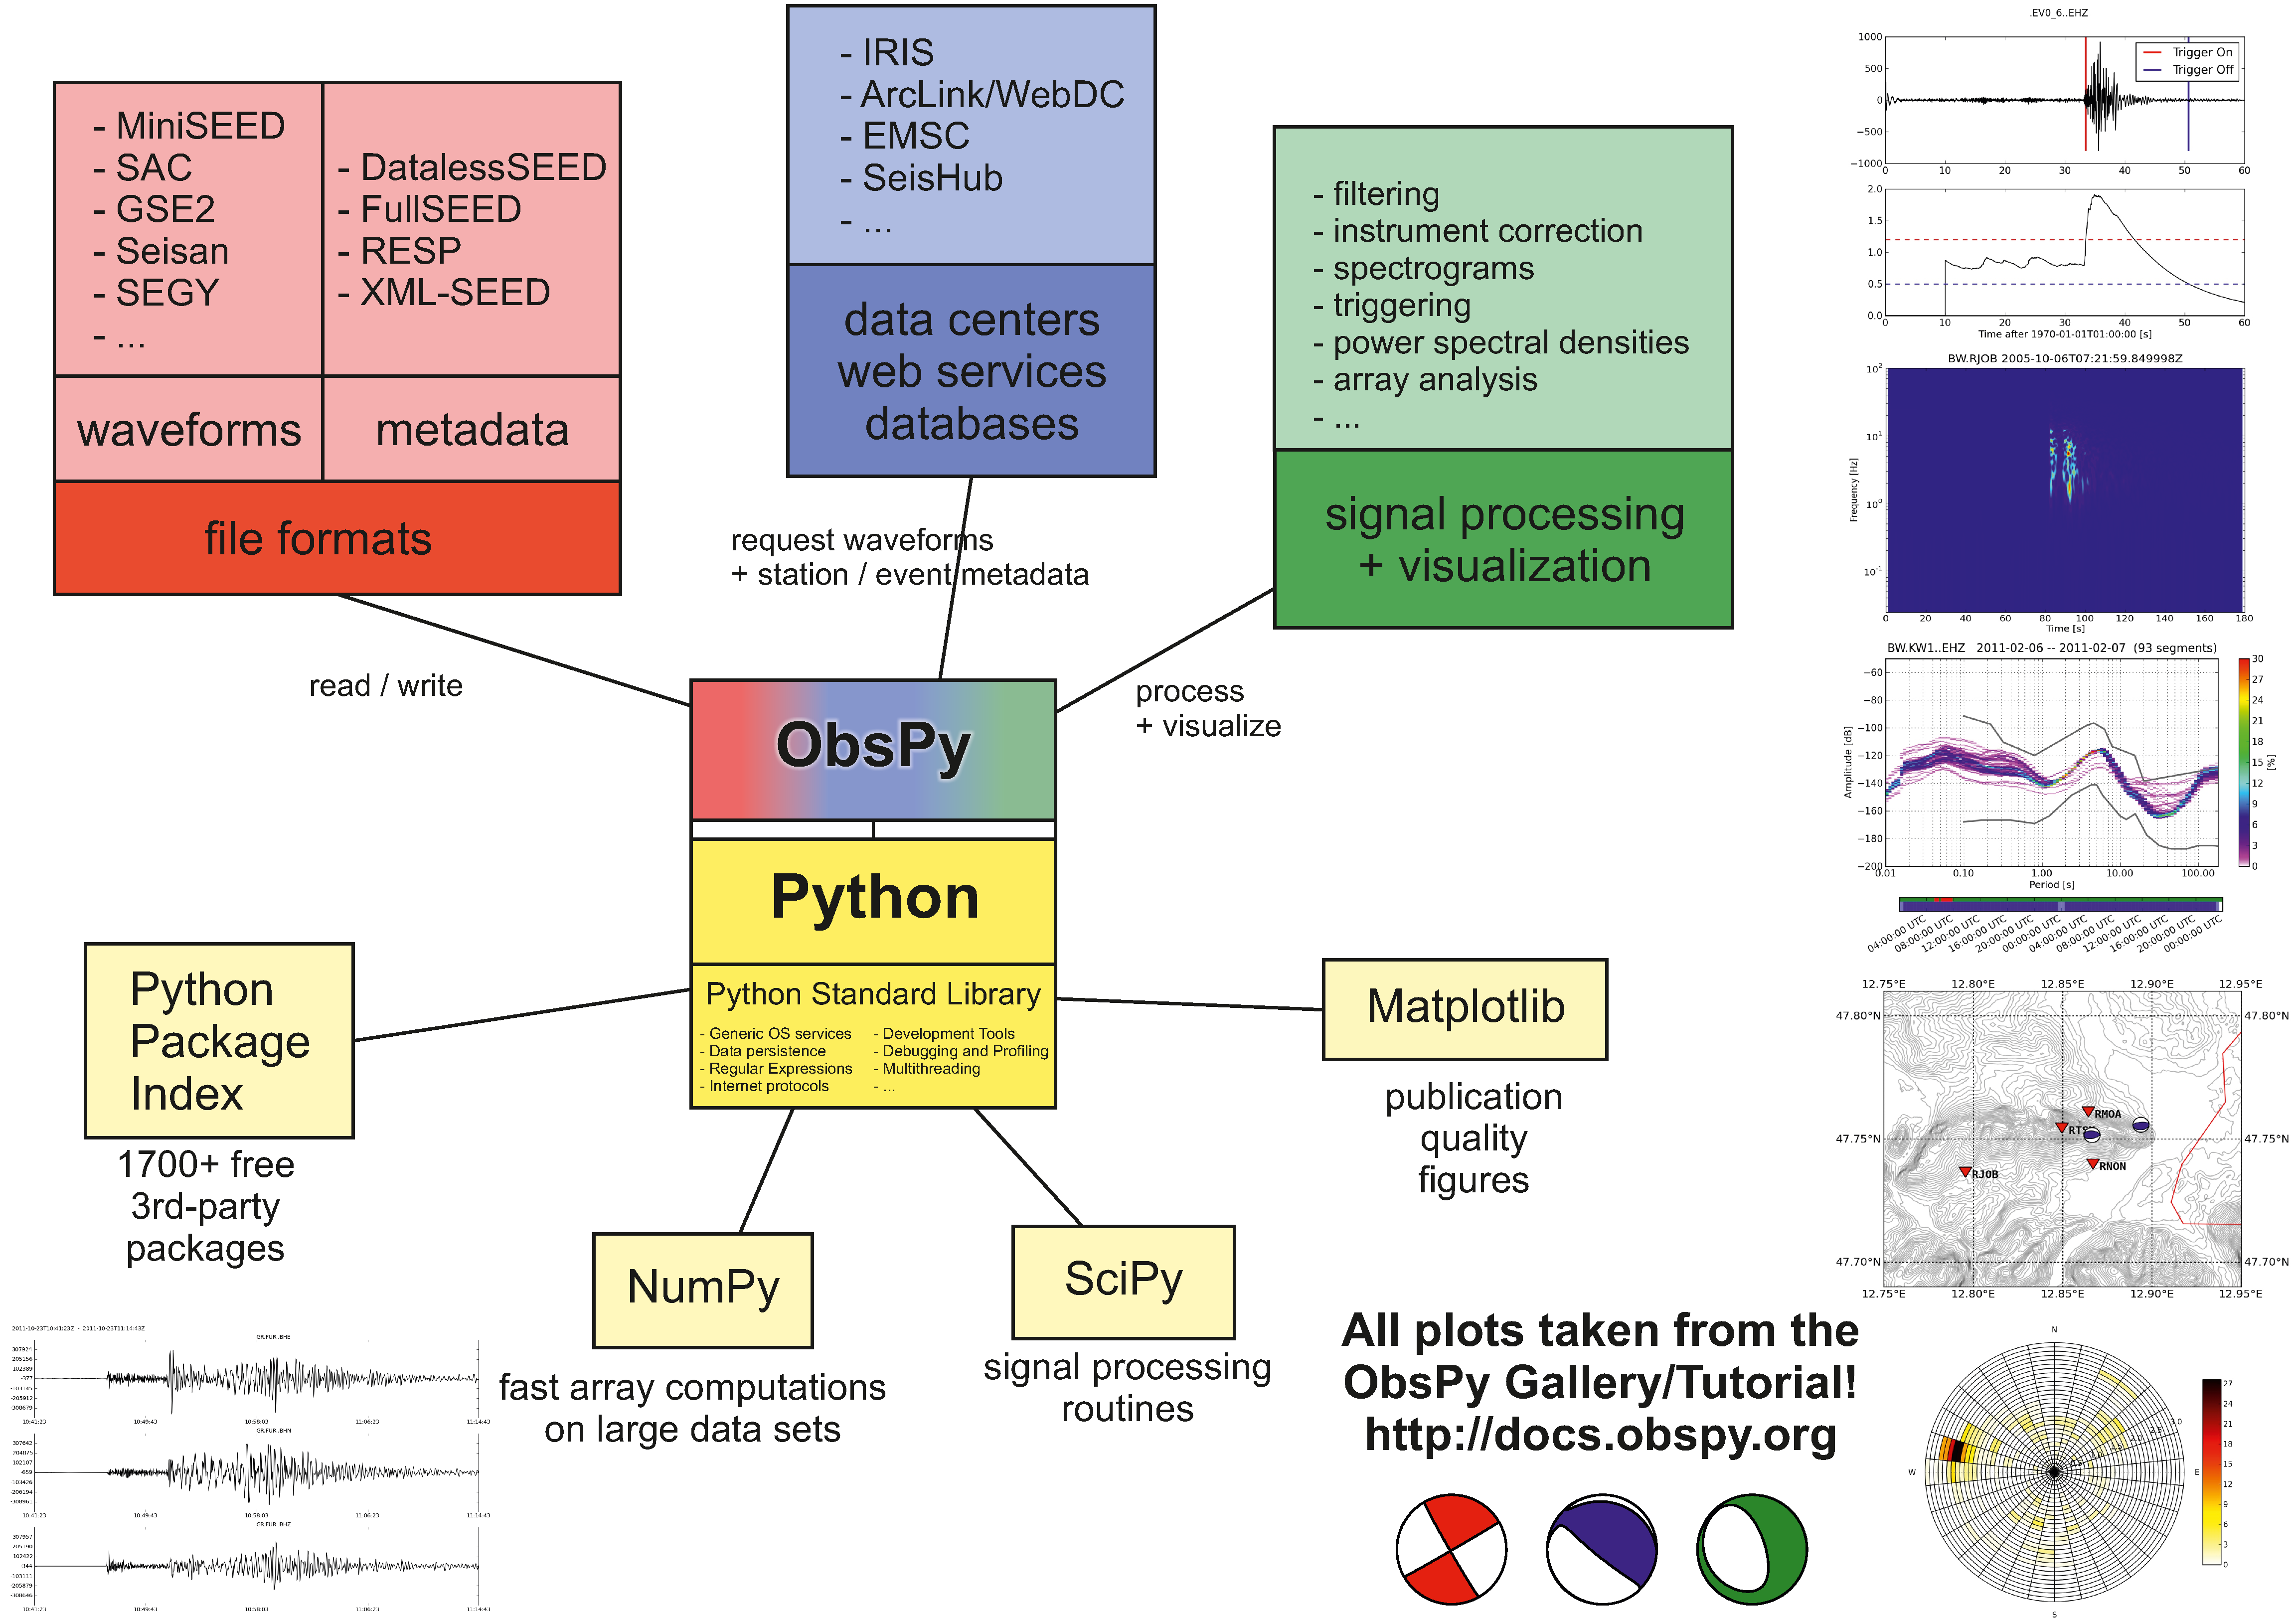
\includegraphics[width=1.00\columnwidth]{obspy.pdf}
}\vspace{0.5\MyBoxVSep}

\MyBox[1em]{
\section*{References}
\large
B\textsc{eyreuther}, M., R. B\textsc{arsch}, L. K\textsc{rischer}, T. M\textsc{egies}, Y. B\textsc{ehr} and J. W\textsc{assermann} (2010)\\
\vspace{0.7cm}
\hspace*{7cm}\textbf{ObsPy: A Python Toolbox for Seismology}, Seismological Research Letters, 81(3):530-533r. doi:10.1785/​gssrl.81.3.530\\
M\textsc{egies}, T., M. B\textsc{eyreuther}, R. B\textsc{arsch}, L. K\textsc{rischer} and J. W\textsc{assermann} (2011)\\
\hspace*{7cm}\textbf{ObsPy – What can it do for data centers and observatories?}. Annals Of Geophysics, 54(1), 47-58. doi:10.4401/ag-4838
\vspace*{0.2cm}
}\vspace{0.5\MyBoxVSep}

\columnbreak
\vspace*{70cm}
%\MyBox[8em]{
%\section*{References}
%}


%\vspace*{7.0\MyBoxHeight}

\end{multicols}
\end{document}
